%
% File: chapters/chapter02/main.tex
% Chapter 2: System Architecture and Data Engineering
%
\chapter{System Architecture and Data Engineering}
\label{chap:02}
\setlength{\parskip}{1em}

\section{Architectural method}

\subsection{Five sibling codebases}

The system is decomposed across five sibling codebases: \texttt{backend/} (Django REST API plus Celery workers), \texttt{mobile/} (React Native client using Expo), \texttt{frontend/} (React + Vite web client for landing and marketing), \texttt{infrastructure/} (Terraform modules and environment configurations), and a separate sibling repository \texttt{etl-meals/} for the ETL pipeline. This decomposition is the subject of ADR-0001 in Chapter~\ref{chap:04}. The first four directories live in a single monorepo so that a pull request can touch backend, mobile, and infrastructure together when the API contract changes, reviewers see the full picture in one place, and CI scopes per-directory path filters so that backend changes do not trigger mobile builds. The ETL pipeline lives in a sibling repository because it depends on heavier machine-learning libraries (sentence-transformers, scrapy, datasets) that do not belong in the production runtime image.

\subsection{C4 model at three levels}

The architecture is documented as a C4 model at three levels. The system context (Level~1) places the meal planner between household users, the operator and administrator, app store reviewers, AWS, and external services (USDA, Spoonacular, Hugging Face, Sentry, PostHog, and Apple/Google push gateways). The container view (Level~2) shows the Django web service (Gunicorn behind ALB), Celery worker and beat (queues: \texttt{default}, \texttt{planning}, \texttt{push}), the RDS Postgres Multi-AZ instance, ElastiCache Redis (cache plus broker on distinct logical databases), S3 media and static buckets fronted by CloudFront, Secrets Manager, the ETL pipeline, the Expo push service, and the two client containers (mobile and web). The component view (Level~3), shown later in Figure~\ref{fig:c4-planning}, zooms into the planning service: the API endpoint dispatches to either an inline synchronous path or a \texttt{PlanGenerationRun} record with a Celery enqueue; the orchestrator constructs the candidate pool, runs scoring (deterministic or ML), invokes the CP-SAT model with a deterministic fallback, builds the shopping list, emits explanations, persists the result, and triggers an Expo push to the requesting user. The Mermaid sources are maintained alongside the running code so that the diagrams cannot drift from the implementation.

\begin{figure}[H]
\centering
\IfFileExists{figures/c4/c4-context.png}{%
  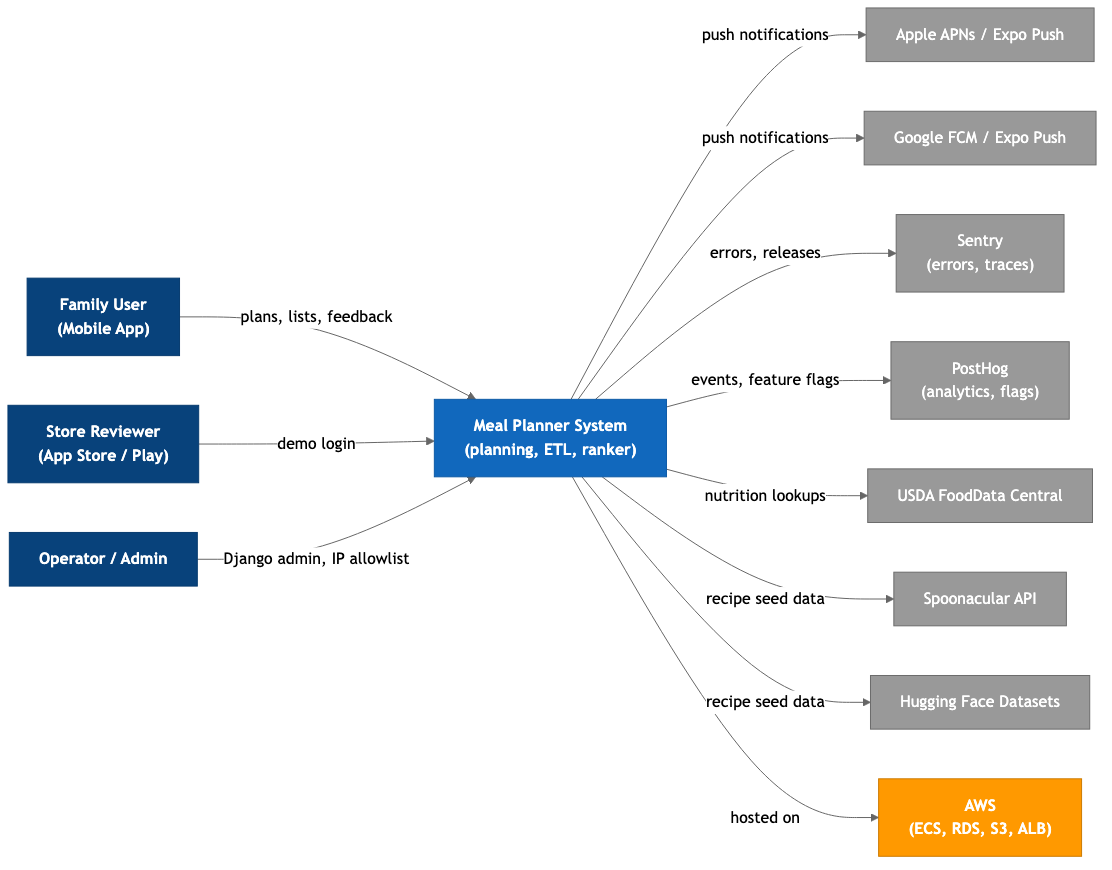
\includegraphics[width=0.95\textwidth]{figures/c4/c4-context.png}%
}{%
  \fbox{\parbox[c][6cm][c]{0.9\textwidth}{\centering Placeholder: \texttt{figures/c4/c4-context.png}}}%
}
\caption{C4 Level~1 --- system context.}
\label{fig:c4-context}
\end{figure}

\begin{figure}[H]
\centering
\IfFileExists{figures/c4/c4-container.png}{%
  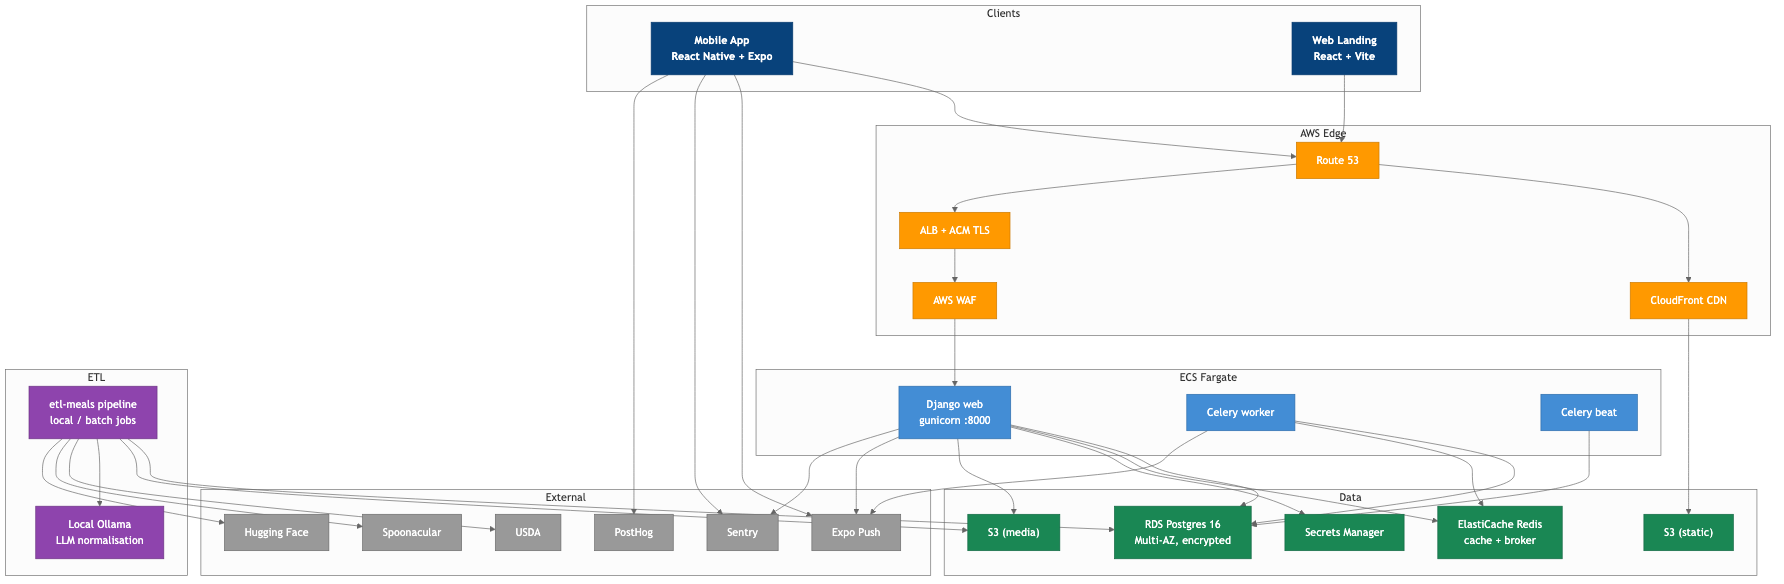
\includegraphics[width=0.95\textwidth]{figures/c4/c4-container.png}%
}{%
  \fbox{\parbox[c][6cm][c]{0.9\textwidth}{\centering Placeholder: \texttt{figures/c4/c4-container.png}}}%
}
\caption{C4 Level~2 --- deployable containers and managed services.}
\label{fig:c4-containers}
\end{figure}

\section{Domain modelling}

\subsection{Application boundaries}

The backend is split into seven Django apps so that coupling stays low and domain boundaries are explicit. The \texttt{users} app owns authentication, profile, settings, and the account lifecycle (delete, export) with Argon2 password hashing and JWT rotation. The \texttt{groups} app models households, members, constraints, and planning preferences. The \texttt{catalog} app owns recipes, canonical ingredients, prices, nutrition, tags, favourites, substitutions, recipe versions, and provenance. The \texttt{planning} app owns plan generation, day items, shopping lists, plan explanations, run records, pantry items, share links, and adaptations. The \texttt{feedback} app owns recipe feedback, plan feedback, interaction events, and notifications. The \texttt{devices} app owns Expo push tokens. The \texttt{common} app provides cross-cutting infrastructure (request-ID middleware, structured logging, throttling, exception handler, response helpers, push helpers, app-version gate, health endpoints, pagination, cache, and an analytics shim).

\subsection{Entity inventory}

Across these apps, the domain is captured by thirty-two persisted entities. Table~\ref{tab:entities-full} enumerates the owner app and purpose of each entity, while Figure~\ref{fig:er} visualises the most important relationships using Mermaid \texttt{erDiagram} notation. The Mermaid source lives under \texttt{docs/diploma/diagrams/er-overview.mmd}; for an exhaustive auto-generated dump including every column, the alternative \texttt{python manage.py graph\_models -a -o schema.png} command from \texttt{django-extensions} can be used.

\begin{longtable}{|l|l|p{8cm}|}
\caption{Persisted domain entities by Django app.}
\label{tab:entities-full}\\
\hline
App & Entity & Purpose \\
\hline
\endfirsthead
\hline
App & Entity & Purpose \\
\hline
\endhead
users    & User                  & Authentication principal (email-as-login) \\
users    & UserSettings          & Notifications, measurement system, currency \\
groups   & Group                 & Household with budget, region, planning defaults \\
groups   & GroupMember           & Member with goal and macro targets \\
groups   & MemberConstraint      & Allergies, religious bans, dislikes \\
groups   & GroupPreference       & Cooking time, repeat tolerance, scalar weights \\
catalog  & Tag                   & Recipe tag with key and label \\
catalog  & Ingredient            & Canonical ingredient \\
catalog  & IngredientPrice       & Regional price reference \\
catalog  & IngredientSubstitution& Substitution candidates with reason \\
catalog  & Recipe                & Recipe with quality score and metadata \\
catalog  & RecipeTag             & Recipe-to-tag link \\
catalog  & RecipeStep            & Recipe instruction step \\
catalog  & RecipeIngredient      & Recipe-to-ingredient link with quantity and unit \\
catalog  & RecipeNutrition       & Per-serving and total macros \\
catalog  & FavoriteRecipe        & User favourite \\
catalog  & RecipeVersion         & Snapshot for audit \\
planning & MealPlan              & Plan with horizon, scores, optimiser metadata \\
planning & MealPlanDay           & Daily bucket \\
planning & MealPlanItem          & Recipe assigned to a (day, meal) slot \\
planning & MealItemAdaptation    & Per-member adaptation suggestion \\
planning & ShoppingList          & Aggregated procurement artifact \\
planning & ShoppingListItem      & Single shopping line \\
planning & PlanExplanation       & Human-readable plan rationale \\
planning & PlanGenerationRun     & Asynchronous run record \\
planning & PantryItem            & Pantry item with optional expiry \\
planning & ShareLink             & Read-only public link \\
feedback & RecipeFeedback        & Like, dislike, or rating with reason \\
feedback & PlanFeedback          & Multi-axis satisfaction \\
feedback & InteractionEvent      & Generic auditable interaction \\
feedback & Notification          & In-app notification \\
devices  & Device                & Expo push token with platform metadata \\
\hline
\end{longtable}

\begin{figure}[H]
\centering
\IfFileExists{figures/er/er-overview.png}{%
  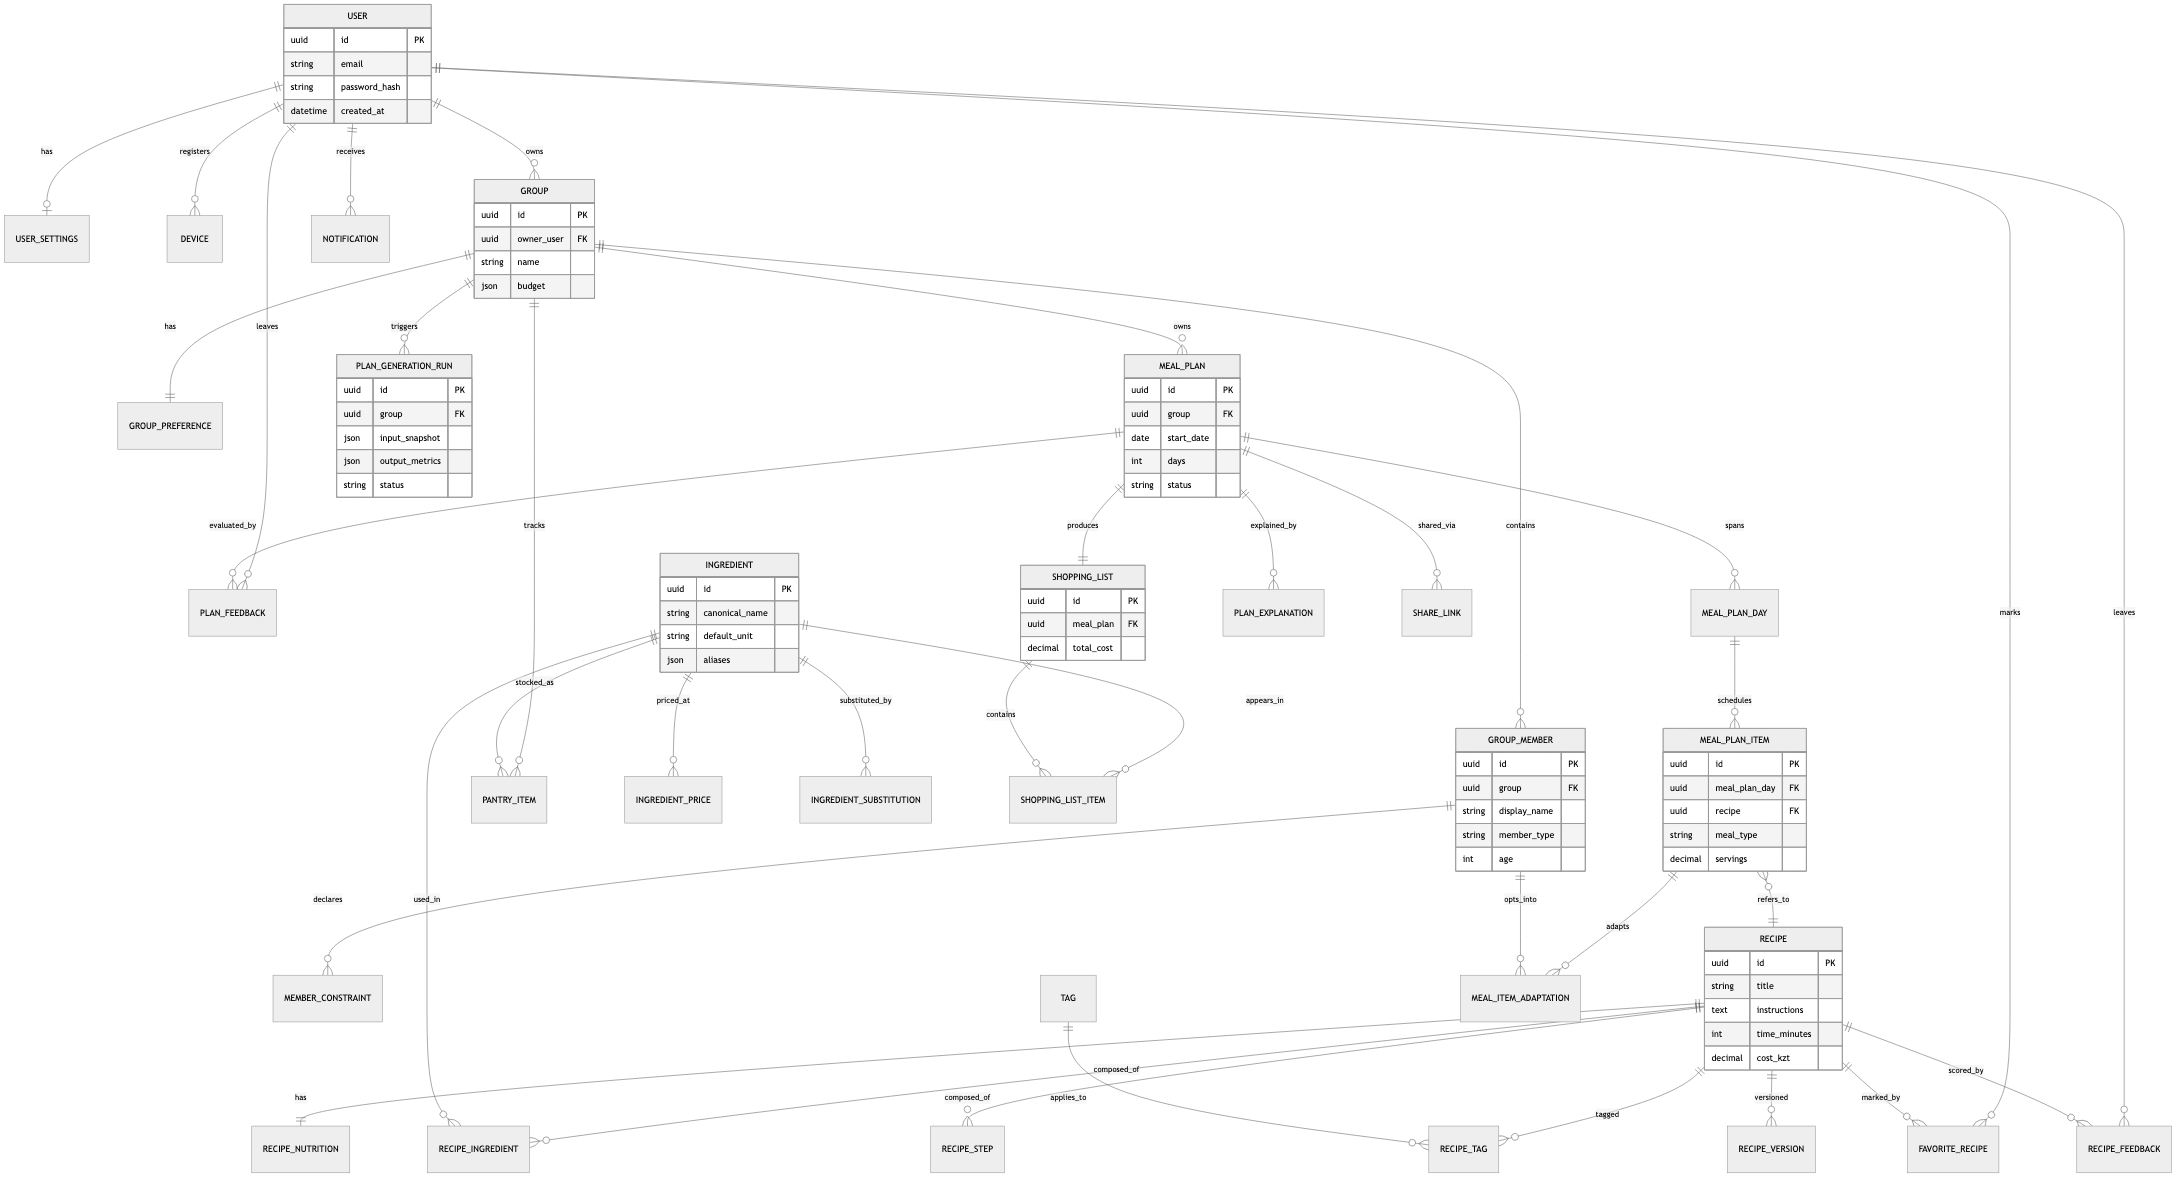
\includegraphics[width=\textwidth,height=0.85\textheight,keepaspectratio]{figures/er/er-overview.png}%
}{%
  \fbox{\parbox[c][6cm][c]{0.9\textwidth}{\centering Placeholder: \texttt{figures/er/er-overview.png}}}%
}
\caption{Domain ER overview across users, groups, catalog, planning, feedback, and devices apps. Audit-only and link tables are omitted for visual clarity.}
\label{fig:er}
\end{figure}

\subsection{Methodological principle}

The methodological principle is explicit representation of planning-critical concepts to improve traceability, testability, and cross-layer consistency. For example, \texttt{Group} represents a household-level planning context with budget, planning defaults, region, and activation state; \texttt{GroupMember} stores per-member demographic and goal data required to derive daily calorie and macro targets; \texttt{MemberConstraint} captures explicit prohibitions and dislikes via ingredient identifiers, tag keys, or free-text values; \texttt{Ingredient} functions as the canonical junction point between price, nutrition, shopping aggregation, and recipe mapping; \texttt{Recipe} stores the primary meal candidate metadata and acts as the anchor for steps, ingredients, tags, and nutrition; \texttt{MealPlan} stores plan-level optimiser metadata, overall scores, budget fit, and nutrition fit; \texttt{MealPlanItem} represents the actual selected meal in a day-slot pair, including cost, calories, servings, and a reason summary; and \texttt{ShoppingList} materialises plan output as an aggregated procurement artifact.

This entity structure also improves integration across layers. ETL outputs can be mapped to stable backend identifiers, planner constraints can reference explicit household and ingredient objects, and frontend analytics can read persisted plan artifacts without inferring hidden state. Changes in one layer can be propagated through predictable model boundaries rather than through ad hoc glue logic.

\section{Reproducible bootstrap}

Reproducibility is treated as an engineering objective in its own right. The backend repository includes versioned data files (\texttt{recipes\_enriched.jsonl}, \texttt{prices-stat.csv}, \texttt{prices\_arbuz.jsonl}, \texttt{nutrition\_catalog.yaml}), Docker Compose configuration, an environment template, and a bootstrap command that orchestrates eight ordered steps. As a result, another developer can rebuild a fresh local database that is functionally equivalent to the authors' environment without depending on a private database dump. For full-scale demonstration, an alternative path imports the production-shaped dump (approximately ninety thousand recipes) via \texttt{pg\_restore}. Both paths converge on a planner-ready state.

The bootstrap command itself is shown in Listing~\ref{lst:bootstrap}.

\begin{lstlisting}[caption={Eight-step bootstrap orchestrated by \texttt{bootstrap\_demo\_data}.},label={lst:bootstrap}]
# Step 1: Import recipes from the enriched JSONL.
python manage.py import_recipes_enriched data/recipes_enriched.jsonl

# Step 2: Import official Kazakh statistical prices.
python manage.py import_stat_prices data/prices-stat.csv

# Step 3: Backfill heuristic prices for ingredients that lack rows.
python manage.py backfill_heuristic_prices

# Step 4: Normalise priority ingredient links (apply).
python manage.py normalize_priority_ingredient_links --apply

# Step 5: Repair suspicious heuristic price rows.
python manage.py repair_heuristic_prices

# Step 6: Repair suspicious recipe unit values.
python manage.py repair_recipe_units --apply

# Step 7: Recalculate cached recipe costs from current ingredient prices.
python manage.py recalculate_recipe_costs

# Step 8: Backfill per-recipe nutrition from the USDA catalog.
python manage.py backfill_recipe_nutrition data/nutrition_catalog.yaml
\end{lstlisting}

\subsection{Reproduce-from-scratch commands}

The complete local reconstruction path starts from containers, runs migrations, creates the operator account, and then invokes the same bootstrap orchestration. Listing~\ref{lst:bootstrap-e2e} is the command sequence used for a clean backend environment.

\begin{lstlisting}[caption={End-to-end bootstrap from versioned data files.},label={lst:bootstrap-e2e}]
cd backend
docker compose up -d --build
docker exec -it meal_planner_backend python manage.py migrate
docker exec -it meal_planner_backend python manage.py createsuperuser
docker exec -it meal_planner_backend python manage.py bootstrap_demo_data \
  --recipes-path data/recipes_enriched.jsonl \
  --prices-path data/prices-stat.csv \
  --nutrition-path data/nutrition_catalog.yaml
\end{lstlisting}

For a full-scale demonstration, the production-shaped dump path restores the larger corpus before the same planner and analytics code is exercised:

\begin{lstlisting}[caption={Full-scale corpus restore from the production-shaped dump.},label={lst:restore-full-corpus}]
docker cp meal_planner.dump meal_planner_postgres:/tmp/dump
docker exec meal_planner_postgres pg_restore \
  -U meal_user -d meal_planner \
  --clean --if-exists --no-owner --no-privileges \
  /tmp/dump
docker exec meal_planner_postgres \
  psql -U meal_user -d meal_planner \
  -c "SELECT COUNT(*) FROM catalog_recipe;"
\end{lstlisting}

The documentation artifacts are reproducible as well. The ER diagram can be regenerated from Django models, while the evaluation charts in Chapter~\ref{chap:04} are rebuilt from the bootstrap data and representative scenario:

\begin{lstlisting}[caption={Regenerate the ER diagram for documentation.},label={lst:regen-er}]
docker exec -it meal_planner_backend pip install django-extensions
docker exec -it meal_planner_backend python manage.py graph_models -a \
  -o /app/staticfiles/schema.png
\end{lstlisting}

\begin{lstlisting}[caption={Regenerate the evaluation charts.},label={lst:regen-charts}]
cd docs/diploma
python -m venv .venv && .venv/bin/pip install matplotlib
MPLCONFIGDIR=/tmp/matplotlib-cache .venv/bin/python scripts/build_charts.py
\end{lstlisting}

\section{Data sources landscape}

The catalog combines three classes of sources: public recipe content (scraped HTML and curated public datasets), official local price feeds, and USDA FoodData Central for nutrition reference. The largest single source is the \texttt{ru\_recipes\_93k} Russian-language recipe dataset on Hugging Face, which provides over ninety-three thousand recipe records and serves as the corpus backbone after deduplication and quality filtering. Three supplementary ingestion paths exist for completeness: TheMealDB and Spoonacular through public REST APIs, and additional web sources through a generic scraping pipeline. Source heterogeneity is the norm in this domain, which means the application cannot assume uniform HTML structure or metadata quality. The ETL subsystem isolates this heterogeneity from the backend.

\section{\texttt{etl-meals} pipeline}
\label{sec:etl-meals-pipeline}

The \texttt{etl-meals/} project is the dedicated Extract--Transform--Load pipeline that turns heterogeneous recipe and price inputs into a backend-ready import bundle. It is intentionally kept outside the production backend image: the ETL needs data-science and scraping dependencies, long-running filesystem stages, and optional external API keys, while the backend needs a small, stable runtime. Figure~\ref{fig:etl-pipeline} shows the pipeline as it exists in the repository.

\begin{figure}[H]
\centering
\small
\resizebox{\textwidth}{!}{%
\begin{tabular}{c c c c c c c}
\fbox{\begin{minipage}{3.1cm}\centering\textbf{Discover}\\sitemaps, category pages, explicit URLs\end{minipage}}
& $\rightarrow$ &
\fbox{\begin{minipage}{3.1cm}\centering\textbf{Acquire}\\raw HTML with delays, retries, cache\end{minipage}}
& $\rightarrow$ &
\fbox{\begin{minipage}{3.1cm}\centering\textbf{Extract}\\JSON-LD \texttt{Recipe} or CSS fallback\end{minipage}}
& $\rightarrow$ &
\fbox{\begin{minipage}{3.1cm}\centering\textbf{Silver}\\normalised generic recipes\end{minipage}}
\\[1.2em]
\fbox{\begin{minipage}{3.1cm}\centering\textbf{Datasets}\\\texttt{ru\_recipes\_93k}, RecipeNLG, TheMealDB, Spoonacular\end{minipage}}
& $\rightarrow$ &
\fbox{\begin{minipage}{3.1cm}\centering\textbf{Enrich}\\time, cuisine, category, servings, quality\end{minipage}}
& $\rightarrow$ &
\fbox{\begin{minipage}{3.1cm}\centering\textbf{Normalise}\\ingredients, units, aliases, nutrition, prices\end{minipage}}
& $\rightarrow$ &
\fbox{\begin{minipage}{3.1cm}\centering\textbf{Export}\\JSONL bundle for Django import\end{minipage}}
\end{tabular}%
}
\caption{\texttt{etl-meals} pipeline from discovery and external datasets to the \texttt{diploma\_work} import bundle.}
\label{fig:etl-pipeline}
\end{figure}

The first stage writes \texttt{data/bronze/discovered\_urls.jsonl} and \texttt{data/bronze/errors.jsonl}; the second preserves raw content so parser improvements can be replayed without re-fetching live websites; the third creates \texttt{data/silver/recipes.jsonl}; and the fourth writes a SQLite warehouse copy for local inspection. The \texttt{export-diploma} command then projects the generic recipe model into the backend catalog schema. The export bundle contains \texttt{tags.jsonl}, \texttt{ingredients.jsonl}, \texttt{ingredient\_prices.jsonl}, \texttt{recipes.jsonl}, \texttt{recipe\_ingredients.jsonl}, \texttt{recipe\_steps.jsonl}, \texttt{recipe\_nutrition.jsonl}, \texttt{recipe\_tags.jsonl}, \texttt{recipe\_sources.jsonl}, \texttt{issues.jsonl}, and \texttt{manifest.json}. The manifest records the target name, source path, primary keys for each table-shaped file, and summary counts.

In the repository snapshot used for this thesis, \texttt{data/silver/recipes.jsonl} contains 90{,}605 generic recipes and \texttt{data/silver/recipes\_enriched.jsonl} contains the same count after enrichment. The \texttt{diploma\_work} export bundle contains 5{,}605 recipe rows, 48{,}703 recipe-ingredient rows, 33{,}880 recipe-step rows, 2{,}307 canonical ingredient rows, 10 tag rows, and a manifest with 103{,}975 issue records. These issues are not runtime failures; they are structured audit notes for approximate unit conversions, low-confidence ingredient parsing, and missing optional enrichment fields. The backend bootstrap sample under \texttt{backend/data/} intentionally uses a smaller 5{,}000-row recipe snapshot for fast local reproduction, while the full silver corpus remains available for production-shaped demonstrations.

The important engineering property of this pipeline is that every handoff is file-based and deterministic. A change to CSS selectors, ingredient parsing, or price heuristics can be re-run from the nearest prior stage, compared by JSONL diffs, and imported into Django only after the manifest and issue file are inspected. This is why ETL is not merely a data-loading script in the project: it is the quality gate that makes planner output explainable, auditable, and reproducible.

\section{URL discovery, acquisition, and extraction}

\subsection{Discovery and raw acquisition}

The discovery stage receives sitemaps, category pages, and explicit URL lists and produces lists of candidate recipe URLs. For source-specific constraints, regular expressions and substring filters reject non-recipe pages. Raw HTML acquisition is performed by an HTTP client with per-host request delays, retry policy, and persistent caching. Preserved HTML enables deterministic re-parsing later, which improves observability: parsing improvements can be tested against historical content without re-fetching live sites.

\subsection{Schema extraction with fallback}

The extraction stage prefers JSON-LD \texttt{schema.org/Recipe} metadata when the source exposes it; CSS-based selectors fall back when it does not. Generic recipe objects are produced with title, ingredient strings, instructions, total time, yields, image, video, cuisine, category, language, and keywords. A subsequent metadata enrichment stage applies rule-based inference to fix missing or inconsistent values: estimating preparation and cooking time from instructions, inferring cuisine and category from titles and ingredient sets, and normalising servings. For unusual cases, optional LLM-assisted normalisation delegates to a local Ollama instance running an open-weight model; the LLM is constrained to deterministic re-formatting tasks and never introduces new factual content.

\section{Canonical ingredient normalisation}

Canonical ingredient normalisation is the most important engineering method in the ETL because prices, nutrition, and shopping-list aggregation all depend on stable ingredient identifiers. Without normalisation, the same ingredient appears under many incompatible forms and joins fail.

The project uses canonical ingredient catalogs, alias-based matching, normalisation reports stored as JSON artifacts, heuristic repairs, and targeted post-import link normalisation through dedicated management commands. This multi-step method reflects the practical reality that no single parser pass is sufficient for noisy recipe data. Measurement unit normalisation is treated separately: unit mismatches were the dominant source of distorted cost estimates in early iterations, and the project adopted explicit repair commands (\texttt{repair\_recipe\_units}, \texttt{repair\_heuristic\_prices}) instead of repeatedly rebuilding the entire catalog.

\section{Embedding-based clustering and MinHash deduplication}

Hand-curating ingredient aliases at the scale of tens of thousands of recipes is not feasible. The project therefore bootstraps ingredient clusters using sentence-transformer embeddings followed by $k$-means clustering. Output clusters are then reviewed and promoted to the canonical alias map. The combination of embedding-based candidate generation with human-in-the-loop confirmation is consistent with general guidance on production ML systems: automation handles scale, while a review step prevents brittle silent failures \cite{sculley2015}.

Duplicate recipes inevitably appear in a multi-source corpus. The same dish (for example, ``classical borscht'') appears under several closely related titles, sometimes with minor ingredient differences. The project uses MinHash with locality-sensitive hashing over ingredient sets to detect near-duplicates. Detected duplicates are demoted to draft status in the backend so that the planner consumes the canonical survivor. This preserves traceability without losing potentially useful provenance.

\section{Quality scoring}

A composite quality score in $[0, 1]$ is computed per recipe across eight components: nutrition coverage, ingredient match ratio, total-time presence, yields presence, image presence, step count, parsed-unit ratio, and price-coverage ratio. The backend persists both the scalar \texttt{quality\_score} and the per-component breakdown (\texttt{quality\_breakdown}, a JSON field). The planner consumes only recipes above a configurable threshold, which means data-quality decisions are externalised from the optimisation logic.

\section{USDA nutrition synchronisation}

Nutrition is treated at the ingredient level rather than the dish level. The \texttt{etl-meals sync-usda-nutrition} command resolves canonical ingredients against USDA FoodData Central using the API key, then writes a local \texttt{nutrition\_catalog.yaml} keyed by normalised ingredient name. The current catalog contains 107~entries covering staples (salt, sugar, water, broth, mayonnaise, flours, oils, meats, vegetables, dairy, spices). For ingredients whose USDA queries return semantically poor matches, curated overrides are stored under \texttt{source\_type: manual\_usda} so that the choice is auditable. Recipe-level nutrition is reconstructed in the backend by aggregating per-ingredient values, scaled by quantity and unit normalisation. This two-path approach (ETL produces the catalog, backend backfills per recipe) was chosen after early experiments showed that ETL-time recipe-level nutrition was less reliable than backend-side aggregation against normalised links.

\section{Multi-source price ingestion}

Two complementary price feeds are used. The first is an official statistical reference (\texttt{prices-stat.csv}) listing average prices on socially significant food categories across twenty Kazakh cities, dated March~2026. The second is the Arbuz.kz retail snapshot (\texttt{prices\_arbuz.jsonl}) produced by a dedicated scraper. The Arbuz snapshot contains 7030~SKU rows across food categories such as ``Бакалея'' (1200), ``Молочное / яйца'' (1200), ``Кофе, чай, сладости'' (1200), ``Замороженные продукты'' (841), ``Консервация'' (365), ``Колбасы и деликатесы'' (362), ``Рыба и морепродукты'' (324), ``Мясо и птица'' (296), and ``Овощи / фрукты'' (291), with units distributed as g~(5186), kg~(755), ml~(557), pc~(357), and l~(175). The statistical reference acts as the citable baseline; the Arbuz snapshot fills the long tail. Both feeds are imported into the backend through \texttt{import\_stat\_prices} and \texttt{import\_market\_prices} commands. Missing prices are then backfilled heuristically and repaired where the heuristic was suspicious. This layered strategy is consistent with the conclusion of recent applied work on Kazakhstani food economics \cite{sapakova2023application} that locally curated price data are necessary for reliable predictions.

\section{Backend implementation surface}

The backend exposes a versioned API under \texttt{/api/v1/} grouped by business function. Authentication endpoints support sign-up, log-in, refresh, identity (``me''), profile retrieval and update, account deletion, and data export. Group endpoints expose group CRUD, active-group resolution, group activation, member management, preference management, setup summary, member constraints, and the group dashboard. Catalog endpoints expose recipe listing, retrieval, tags, categories, search suggestions, favourites, ingredient listing, and ingredient prices. Planning endpoints expose plan generation, listing, current plan, detailed retrieval, day detail, replacement of a single item, adaptation CRUD, shopping list, shopping-list regeneration, shopping-list custom-item creation and update or delete, pantry-aware shopping list, budget analytics, nutrition analytics, explanations, generation-run polling, approval, archive, clone, delete, price comparison, share-link creation, and public-read view via share token. Feedback endpoints expose recipe and plan feedback creation, interaction event creation, history listings, and notification listing, read, and read-all. Devices endpoints expose Expo token registration, listing, and unregistration. The public surface map is kept in the thesis body because it is part of the implemented system boundary, not supplementary material.

\subsection{Public API surface map}

\paragraph{Authentication and account.}
\begin{itemize}
\item \texttt{/api/v1/auth/sign-up} (POST)
\item \texttt{/api/v1/auth/log-in} (POST)
\item \texttt{/api/v1/auth/log-out} (POST)
\item \texttt{/api/v1/auth/refresh} (POST)
\item \texttt{/api/v1/auth/me} (GET)
\item \texttt{/api/v1/auth/profile} (GET, PATCH)
\item \texttt{/api/v1/auth/account/delete} (POST)
\item \texttt{/api/v1/auth/account/export} (GET)
\item \texttt{/api/v1/profile} (GET, PATCH)
\item \texttt{/api/v1/settings} (GET, PATCH)
\end{itemize}

\paragraph{Groups, members, constraints, preferences.}
\begin{itemize}
\item \texttt{/api/v1/groups} (GET, POST)
\item \texttt{/api/v1/groups/active} (GET)
\item \texttt{/api/v1/groups/\{group\_id\}} (GET, PATCH)
\item \texttt{/api/v1/groups/\{group\_id\}/activate} (POST)
\item \texttt{/api/v1/groups/\{group\_id\}/members} (GET, POST)
\item \texttt{/api/v1/groups/\{group\_id\}/preferences} (GET, PATCH)
\item \texttt{/api/v1/groups/\{group\_id\}/setup-summary} (GET)
\item \texttt{/api/v1/groups/\{group\_id\}/dashboard} (GET)
\item \texttt{/api/v1/members/\{member\_id\}} (GET, PATCH, DELETE)
\item \texttt{/api/v1/members/\{member\_id\}/constraints} (GET, POST)
\item \texttt{/api/v1/constraints/\{constraint\_id\}} (PATCH, DELETE)
\end{itemize}

\paragraph{Catalog, favourites, ingredients.}
\begin{itemize}
\item \texttt{/api/v1/recipes} (GET)
\item \texttt{/api/v1/recipes/tags} (GET)
\item \texttt{/api/v1/recipes/categories} (GET)
\item \texttt{/api/v1/recipes/search-suggestions} (GET)
\item \texttt{/api/v1/recipes/\{recipe\_id\}} (GET)
\item \texttt{/api/v1/favorites/recipes} (GET, POST)
\item \texttt{/api/v1/favorites/recipes/\{recipe\_id\}} (DELETE)
\item \texttt{/api/v1/ingredients} (GET)
\item \texttt{/api/v1/ingredients/\{ingredient\_id\}/prices} (GET)
\end{itemize}

\paragraph{Planning, runs, lifecycle.}
\begin{itemize}
\item \texttt{/api/v1/groups/\{group\_id\}/meal-plans} (GET)
\item \texttt{/api/v1/groups/\{group\_id\}/meal-plans/generate} (POST)
\item \texttt{/api/v1/groups/\{group\_id\}/meal-plans/current} (GET)
\item \texttt{/api/v1/meal-plans/\{meal\_plan\_id\}} (GET)
\item \texttt{/api/v1/meal-plans/\{meal\_plan\_id\}/days/\{day\_index\}} (GET)
\item \texttt{/api/v1/meal-plan-items/\{item\_id\}/replace} (POST)
\item \texttt{/api/v1/meal-plan-items/\{item\_id\}/adaptations} (GET, POST)
\item \texttt{/api/v1/meal-plan-items/\{item\_id\}/adaptations/\{adaptation\_id\}} (PATCH, DELETE)
\item \texttt{/api/v1/meal-plans/\{meal\_plan\_id\}/shopping-list} (GET)
\item \texttt{/api/v1/meal-plans/\{meal\_plan\_id\}/shopping-list/regenerate} (POST)
\item \texttt{/api/v1/meal-plans/\{meal\_plan\_id\}/shopping-list/with-pantry-adjustment} (GET)
\item \texttt{/api/v1/meal-plans/\{meal\_plan\_id\}/shopping-list/custom-items} (POST)
\item \texttt{/api/v1/shopping-list-items/\{item\_id\}} (PATCH, DELETE)
\item \texttt{/api/v1/meal-plans/\{meal\_plan\_id\}/budget-analytics} (GET)
\item \texttt{/api/v1/meal-plans/\{meal\_plan\_id\}/nutrition-analytics} (GET)
\item \texttt{/api/v1/meal-plans/\{meal\_plan\_id\}/explanations} (GET)
\item \texttt{/api/v1/meal-plans/\{meal\_plan\_id\}/generation-run} (GET)
\item \texttt{/api/v1/meal-plans/generation-run/\{run\_id\}} (GET)
\item \texttt{/api/v1/meal-plans/\{meal\_plan\_id\}/approve} (POST)
\item \texttt{/api/v1/meal-plans/\{meal\_plan\_id\}/archive} (POST)
\item \texttt{/api/v1/meal-plans/\{meal\_plan\_id\}/clone} (POST)
\item \texttt{/api/v1/meal-plans/\{meal\_plan\_id\}/delete} (DELETE)
\item \texttt{/api/v1/meal-plans/\{meal\_plan\_id\}/price-comparison} (GET)
\item \texttt{/api/v1/meal-plans/\{meal\_plan\_id\}/share-links} (POST)
\item \texttt{/api/v1/shared/meal-plans/\{share\_token\}} (GET, public)
\item \texttt{/api/v1/groups/\{group\_id\}/pantry-items} (GET, POST)
\item \texttt{/api/v1/pantry-items/\{pantry\_item\_id\}} (PATCH, DELETE)
\end{itemize}

\paragraph{Feedback, history, notifications.}
\begin{itemize}
\item \texttt{/api/v1/recipes/\{recipe\_id\}/feedback} (POST)
\item \texttt{/api/v1/meal-plans/\{meal\_plan\_id\}/feedback} (POST)
\item \texttt{/api/v1/events} (POST)
\item \texttt{/api/v1/groups/\{group\_id\}/history/meal-plans} (GET)
\item \texttt{/api/v1/groups/\{group\_id\}/history/recipes} (GET)
\item \texttt{/api/v1/notifications} (GET)
\item \texttt{/api/v1/notifications/\{notification\_id\}/read} (POST)
\item \texttt{/api/v1/notifications/read-all} (POST)
\end{itemize}

\paragraph{Devices.}
\begin{itemize}
\item \texttt{/api/v1/devices/register} (POST)
\item \texttt{/api/v1/devices} (GET)
\item \texttt{/api/v1/devices/\{device\_id\}} (DELETE)
\end{itemize}

\section{Mobile and web clients}

\subsection{Mobile client}

The mobile client is the primary delivery surface. It is implemented in React Native via the Expo SDK 51 managed workflow, with EAS Build for store binaries and EAS Update for over-the-air JavaScript patches. The decision to use Expo Managed is captured by ADR-0004 (Chapter~\ref{chap:04}). The codebase contains twenty-seven screens organised in six categories: authentication, home, onboarding, planning, profile, and recipes. Navigation is handled by React Navigation (bottom tabs plus stack), with deep linking pre-configured for \texttt{exp://} and \texttt{mealplanner://} schemes. State management is predominantly server-state via TanStack Query, with local form state via React Hook Form. The design system lives in \texttt{shared/ui/theme.ts} and provides palette, spacing, radii, typography, shadows, and motion tokens. All user-interface strings flow through \texttt{shared/lib/formatters.ts} so that Russian pluralisation and label maps are centralised.

\subsection{Onboarding workflow}

The mobile onboarding is intentionally household-centric rather than recipe-centric. The user proceeds through six steps before plan generation is enabled: mode selection (household profile shape), create household (name, region, currency), members (per-member type, age, sex, activity, goal), preferences (spice tolerance, max cooking time, repeat tolerance, variety), budget (amount, period, strictness), and summary (review). Each step persists incrementally so that interrupted onboarding can resume. Constraints (allergies, religious bans, dislikes) are attached per member after the summary step.

\subsection{Plan viewing and explanation}

Once plan generation completes, the user lands on the weekly plan view that lists every day-slot pair with cost, calories, and a thumbnail. Tapping a day opens a detailed view with per-meal cards, an item-level cost breakdown, and per-member adaptation notes. Tapping a recipe opens the recipe detail screen, which renders ingredients (linked to the canonical catalog), step-by-step instructions, and per-serving nutrition. A separate ``explanations'' surface answers \emph{why this plan?} by showing the optimiser's selection rationale (active constraints, scoring components, swap suggestions) so that the recommendation does not feel opaque to the household. Figure~\ref{fig:mobile-plan-screens} captures these four surfaces from the Expo client.

\begin{figure}[H]
\centering
\begin{subfigure}[t]{0.23\textwidth}
  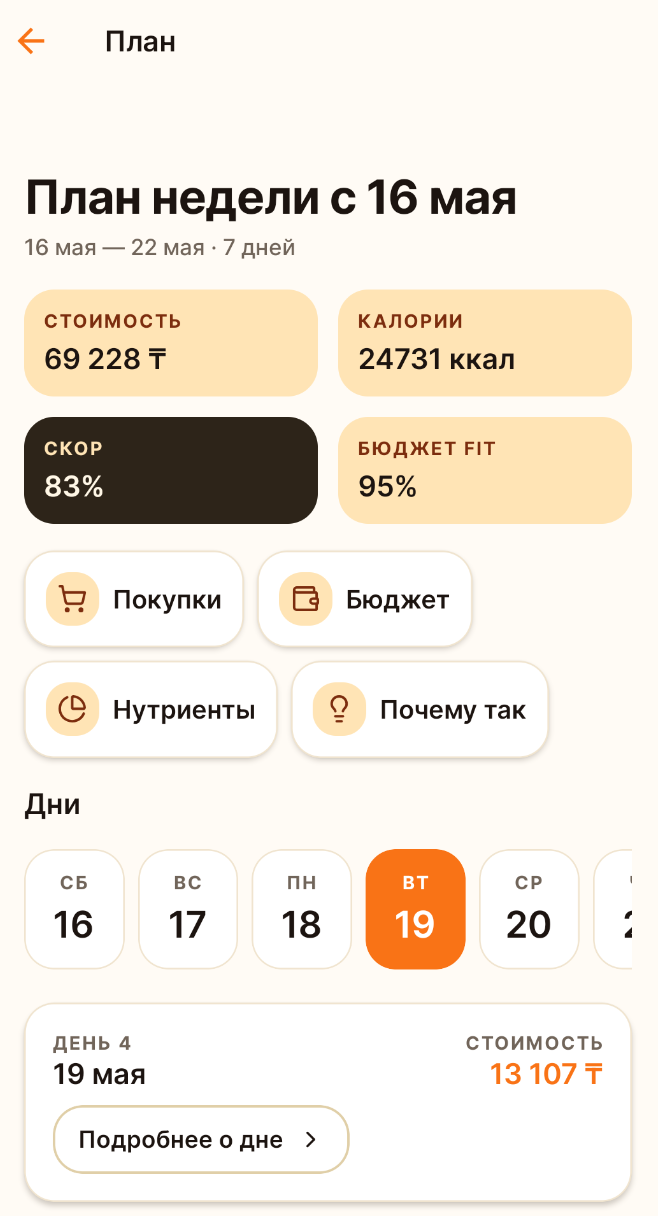
\includegraphics[width=\linewidth]{presentation-assets/screenshots/01-plan-week.png}
  \caption{Weekly plan}
\end{subfigure}\hfill
\begin{subfigure}[t]{0.23\textwidth}
  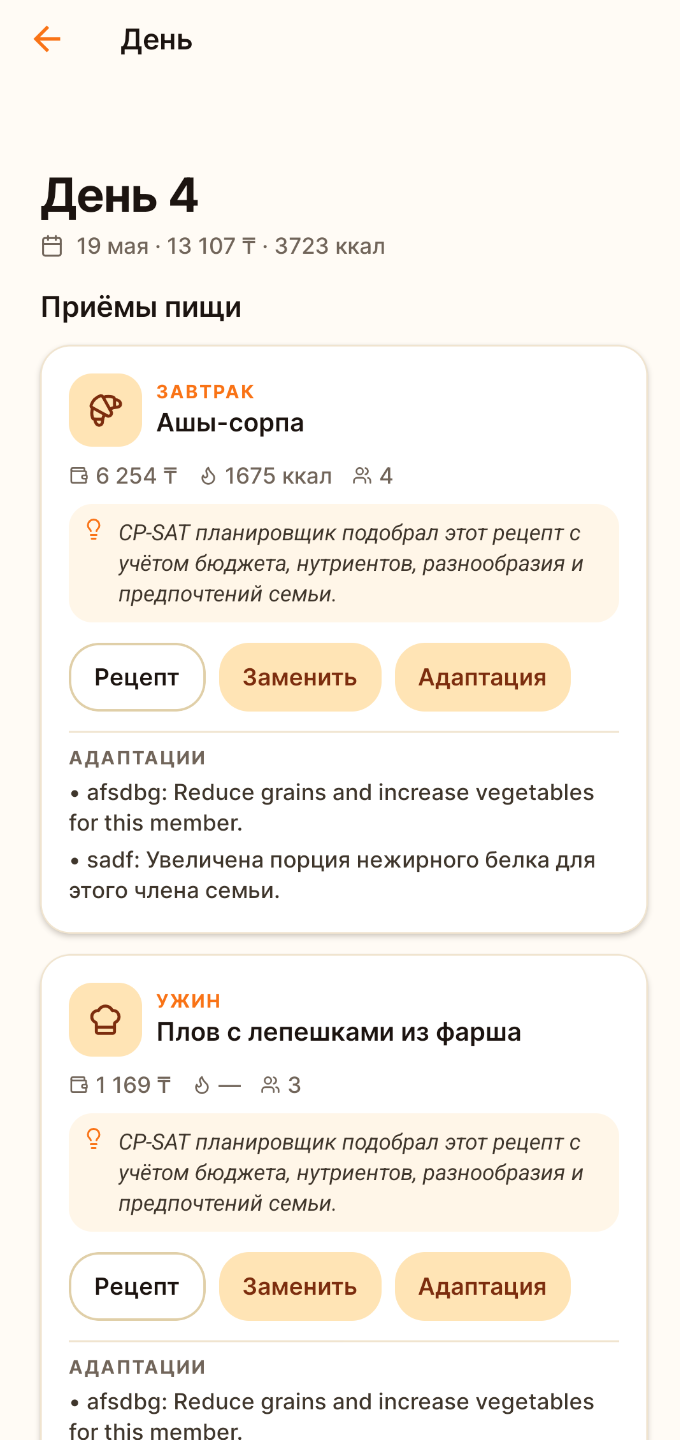
\includegraphics[width=\linewidth]{presentation-assets/screenshots/02-plan-day.png}
  \caption{Daily detail}
\end{subfigure}\hfill
\begin{subfigure}[t]{0.23\textwidth}
  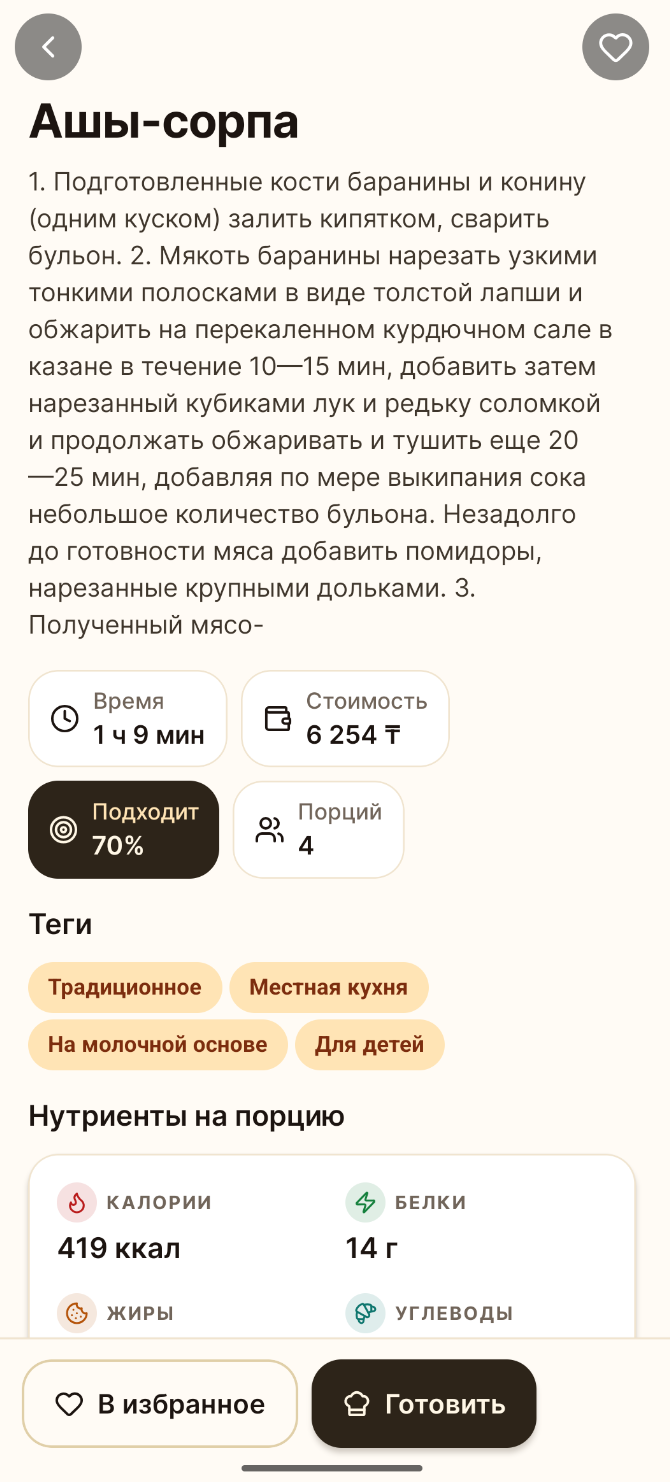
\includegraphics[width=\linewidth]{presentation-assets/screenshots/03-recipe-detail.png}
  \caption{Recipe detail}
\end{subfigure}\hfill
\begin{subfigure}[t]{0.23\textwidth}
  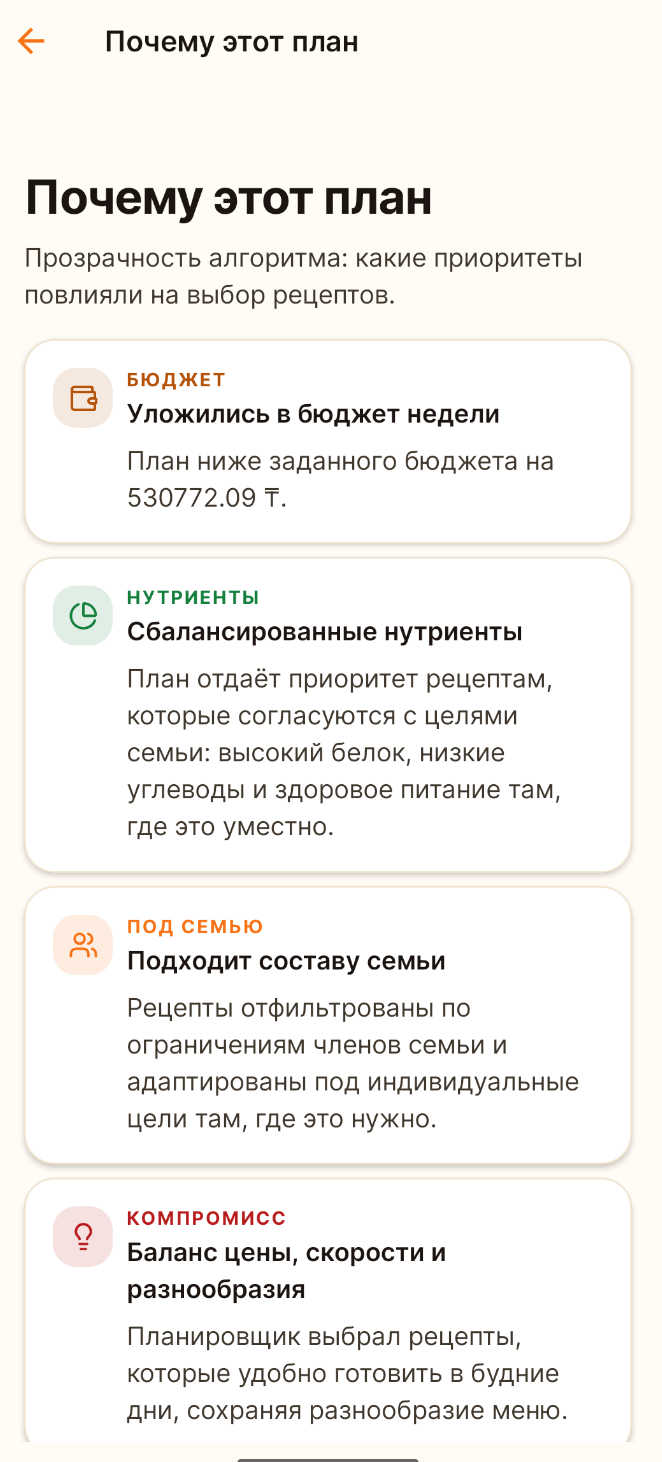
\includegraphics[width=\linewidth]{presentation-assets/screenshots/06-plan-explanation.png}
  \caption{Plan explanation}
\end{subfigure}
\caption{Mobile plan-viewing surfaces: weekly overview, daily detail, recipe detail, and plan explanation.}
\label{fig:mobile-plan-screens}
\end{figure}

\subsection{Analytics, shopping, pantry, and sharing}

Two analytics surfaces summarise plan quality at a glance: the nutrition analytics screen aggregates per-day macros and compares them to per-member targets, while the budget analytics screen breaks the plan cost down by day and by ingredient category, with a clear indicator of slack against the household budget. The shopping list screen renders the aggregated procurement artifact as a tickable list grouped by category, with quantities scaled to the chosen number of servings; the pantry-aware variant subtracts on-hand quantities so the user does not buy what is already available. The pantry screen lets users record items with quantities and optional expiry dates; an add-product modal supports both catalog selection (typed search against canonical ingredients) and free-text entries. Plans can also be shared through a public read-only link that expires and can be deactivated. Figure~\ref{fig:mobile-analytics-pantry-screens} captures these four surfaces.

\begin{figure}[H]
\centering
\begin{subfigure}[t]{0.23\textwidth}
  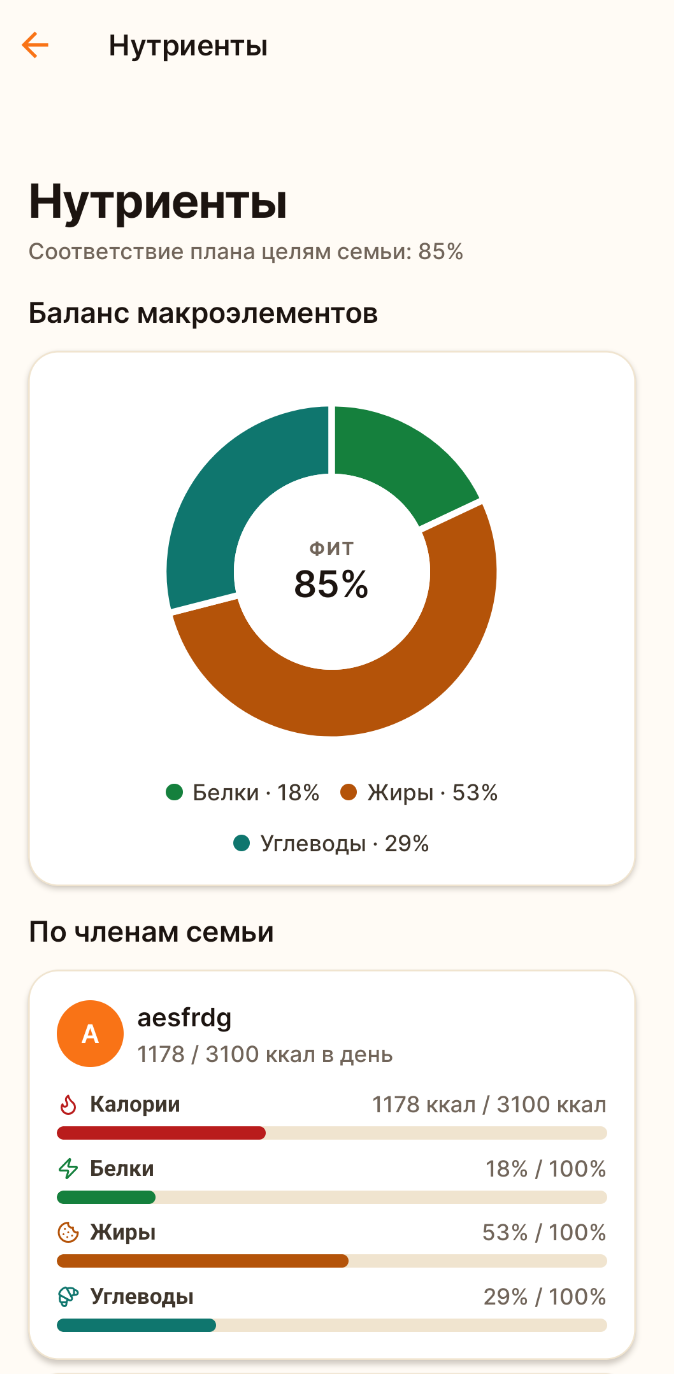
\includegraphics[width=\linewidth]{presentation-assets/screenshots/04-nutrition-analytics.png}
  \caption{Nutrition analytics}
\end{subfigure}\hfill
\begin{subfigure}[t]{0.23\textwidth}
  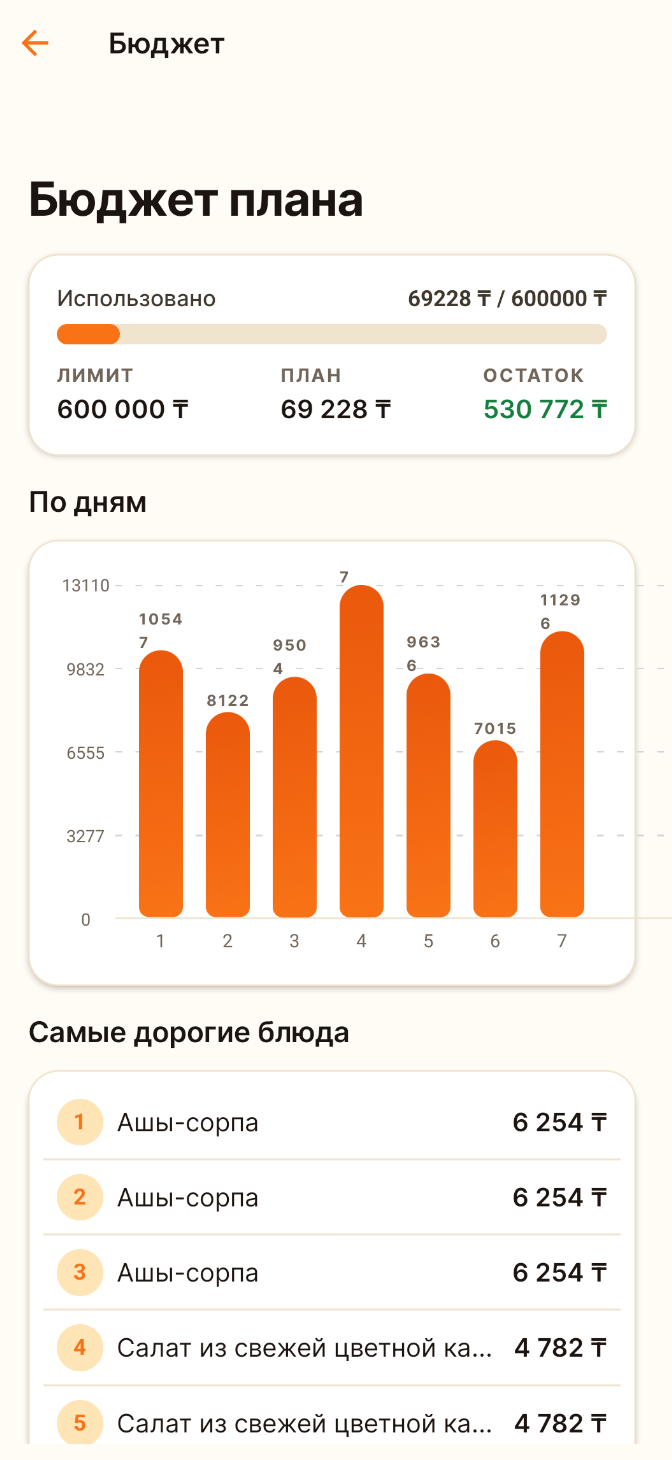
\includegraphics[width=\linewidth]{presentation-assets/screenshots/05-budget-analytics.png}
  \caption{Budget analytics}
\end{subfigure}\hfill
\begin{subfigure}[t]{0.23\textwidth}
  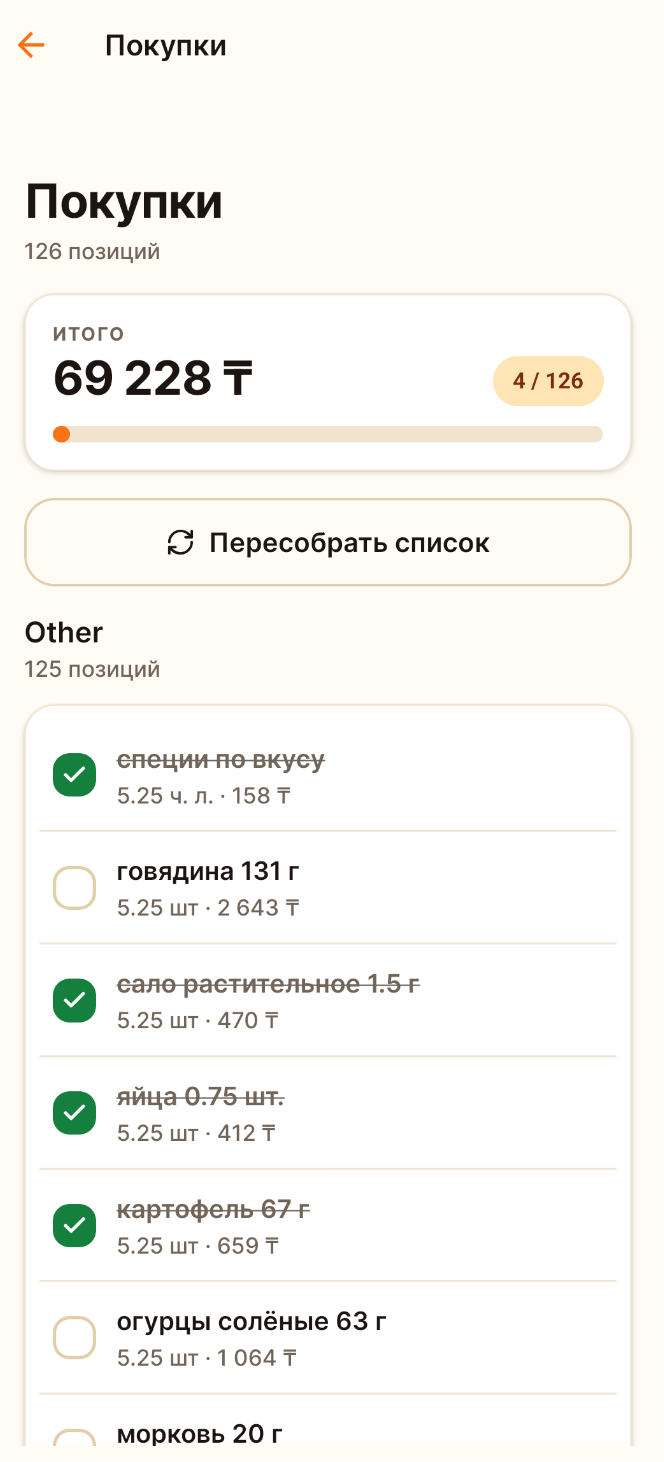
\includegraphics[width=\linewidth]{presentation-assets/screenshots/07-shopping-list.png}
  \caption{Shopping list}
\end{subfigure}\hfill
\begin{subfigure}[t]{0.23\textwidth}
  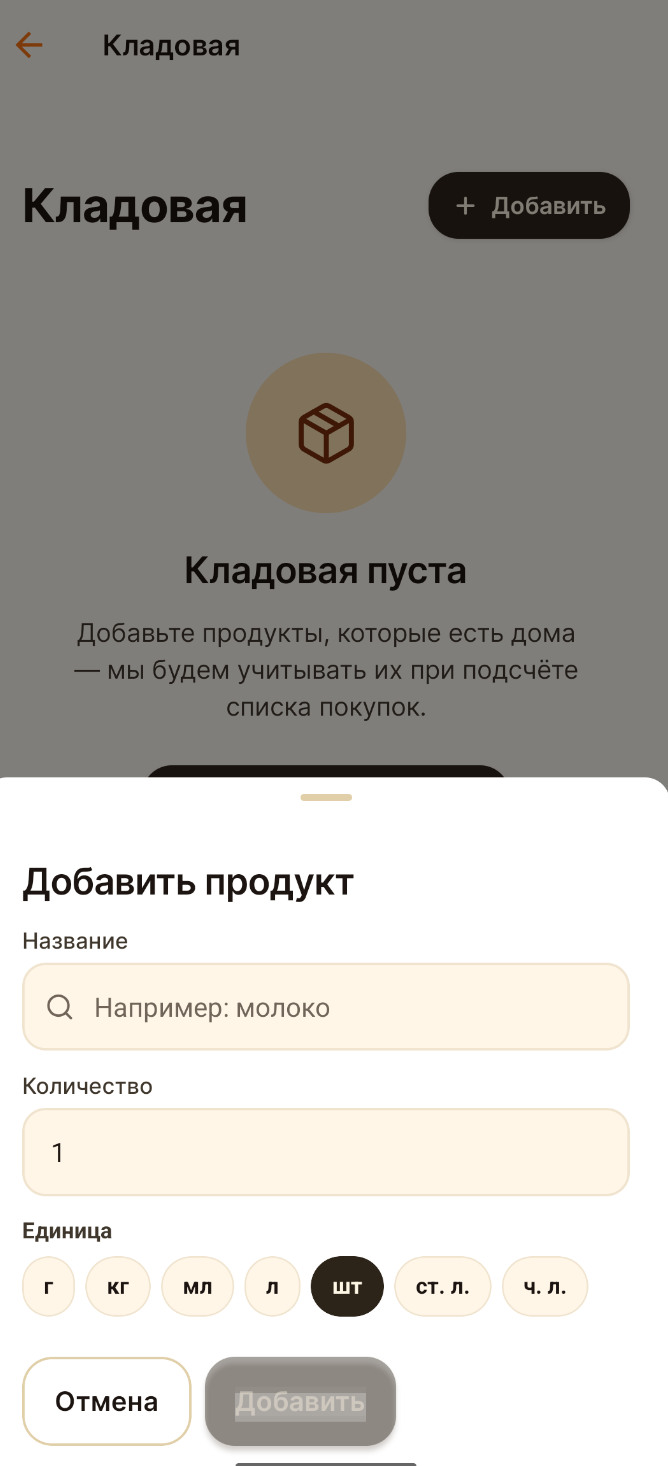
\includegraphics[width=\linewidth]{presentation-assets/screenshots/08-pantry-add-product.png}
  \caption{Pantry add product}
\end{subfigure}
\caption{Mobile analytics, shopping, and pantry surfaces captured from the Expo client.}
\label{fig:mobile-analytics-pantry-screens}
\end{figure}

\subsection{Plan generation, pantry, and sharing}

Plan generation begins on a dedicated screen where the user selects horizon (days), meals per day, optimisation focus (budget, nutrition, speed, taste), and strictness levels for budget and cooking time. Submission triggers an asynchronous pipeline (Section~\ref{sec:async-pipeline}). The screen polls the run state and transitions to the weekly view once the plan is ready (Figure~\ref{fig:mobile-plan-screens}). Pantry items can be recorded with quantities and optional expiry dates (Figure~\ref{fig:mobile-analytics-pantry-screens}); a dedicated pantry-aware shopping-list endpoint subtracts on-hand quantities so that the user does not buy what is already available. A share link can be created for any meal plan and consumed publicly by an anonymous read-only viewer; share links expire and can be deactivated.

\subsection{Feature-Sliced Design in the mobile client}

The mobile codebase follows a Feature-Sliced-Design-inspired layered organisation adapted for React Native. Five top-level layers under \texttt{mobile/src/} are used in the order of decreasing volatility: \emph{core} (Expo navigation root, providers, deep-linking configuration), \emph{screens} (the twenty-seven destinations grouped by area: auth, home, onboarding, plans, profile, recipes), \emph{features} (single-user-intent actions such as ``replace plan item'', ``register Expo push token'', or the onboarding wizard step hooks; organised by domain: auth, catalog, groups, notifications, onboarding, pantry, plans, recipes, settings), \emph{entities} (domain models with their API client, query keys, and view components: \texttt{recipe}, \texttt{plan}, \texttt{group}), and \emph{shared} (design-system tokens, formatters, the typed HTTP client, query-client configuration, error boundaries, telemetry adapters for Sentry and PostHog, and reusable hooks). Imports are intended to flow downward only (a screen may import features, entities, and shared; a feature may import entities and shared; an entity may import only shared); the convention is enforced through code review supported by TypeScript path aliases (\texttt{@core/}, \texttt{@features/}, \texttt{@entities/}, \texttt{@shared/}) defined in \texttt{tsconfig.json}, with a future migration to ESLint boundaries planned. The benefit is that adding a new screen typically reduces to composing existing entities and feature hooks rather than rewriting bespoke views.

The data layer is built around TanStack Query. Each entity exposes a curated set of query keys and hooks: for example, the recipe entity exports \texttt{useRecipeListQuery}, \texttt{useRecipeDetailQuery}, and \texttt{useFavoriteRecipeMutation}. Mutations invalidate the corresponding query keys on success, so the cache stays consistent without explicit refetch calls in the screen. Optimistic updates are applied for favourites and for shopping-item check-off, both because their failure mode is benign and because the user expects immediate visual feedback. Network errors flow through a single \texttt{errorMessageFor()} helper that maps backend error codes to localised messages, so screens never duplicate the same error-handling block.

\subsection{Web client}

The web client is scoped to landing, marketing, and a minimal dashboard that exercises the same API contract as the mobile application. The client uses Vite for development, React for rendering, and TypeScript for contract safety. It is intentionally smaller than the mobile client because product priorities favour mobile for end-user delivery; the web client primarily serves as a public face for users approaching the project from the web and as an integration surface for marketing materials.

\section{Asynchronous planning pipeline}
\label{sec:async-pipeline}

Plan generation is moved off the request path to keep HTTP latency low. The flow is as follows. A client posts to \texttt{/api/v1/groups/<id>/meal-plans/generate}; the API view applies the plan-generation throttle (default twenty requests per hour per user, configurable via the \texttt{DRF\_PLAN\_THROTTLE} environment variable), creates a \texttt{PlanGenerationRun} with status \texttt{pending}, and enqueues the Celery task \texttt{apps.planning.tasks.generate\_meal\_plan\_async} on the \texttt{planning} queue. The worker runs the orchestrator, persists the resulting \texttt{MealPlan}, updates the run record to \texttt{completed} or \texttt{failed}, and triggers an Expo push to the requesting user. The client polls \texttt{/api/v1/meal-plans/generation-run/<run\_id>} until the run completes. The same Celery infrastructure carries three additional periodic tasks: pantry-expiration notifications, recipe-ranker retraining, and recipe-cost recalculation.

\subsection{Celery queue topology and idempotency}

Three named queues are used: \texttt{default} for short, latency-sensitive work (push token registration, notification fan-out, telemetry forwarding), \texttt{planning} for the longer plan-generation pipeline, and \texttt{push} for outbound Expo push delivery. The queues are deployed as two physical worker processes so that a stuck plan-generation run cannot starve push delivery; Celery routing tables are configured statically in \texttt{settings.py} via the \texttt{task\_routes} map. Tasks declare retry policies appropriate to their failure mode: idempotent tasks (push delivery, ranker retraining) use \texttt{autoretry\_for} with exponential backoff and a six-attempt cap, while plan generation is intentionally non-retriable on user-visible failure --- the user retries explicitly from the UI after they see the run state transition to \texttt{failed}, because silent retries would hide intermittent bugs. Idempotency of side effects is enforced through the \texttt{PlanGenerationRun} record: the run id is the natural deduplication key, and the worker checks the current status before performing any expensive work so that a duplicate broker delivery cannot double-write the plan.

\section{API design principles}

The API follows five engineering principles. First, \emph{versioning at the path} (\texttt{/api/v1/}) was chosen over header-based versioning because it is the most easily debugged path for mobile clients: any request seen in CloudWatch logs immediately discloses the contract that produced it. Second, \emph{consistent error envelopes} are required: every non-2xx response includes a JSON body with \texttt{detail}, \texttt{code}, and optional \texttt{field\_errors}; the mobile client maps these to localised messages through a single shared helper. Third, \emph{request correlation} is mandatory: every incoming request is tagged with an \texttt{X-Request-ID} header that is propagated to log records (via \texttt{structlog} contextvars), to Celery task arguments, and to all Sentry breadcrumbs; this means a single user-reported failure can be traced across the web pod, the Celery worker, and the mobile log uniformly. Fourth, \emph{pagination is opt-in but uniform}: list endpoints accept \texttt{page} and \texttt{page\_size}, the response includes \texttt{count}, \texttt{next}, and \texttt{previous}, and the page size is bounded by per-endpoint maxima so that an accidental large request cannot exhaust memory. Fifth, \emph{idempotency for state-changing actions}: plan replacement, shopping-list item check-off, and pantry mutations all accept an optional \texttt{Idempotency-Key} header, which the backend uses to deduplicate retried requests from spotty mobile networks.

The API contract is documented as machine-readable OpenAPI through \texttt{drf-spectacular}. The schema is generated dynamically by the \texttt{SpectacularAPIView} at \texttt{/api/v1/schema/} on every deployment and rendered as a browseable Swagger UI at \texttt{/api/v1/docs/}. The mobile client could consume the schema for code generation; in practice the project keeps a hand-written TypeScript contract synchronised through code review, because the screen-level types deviate from the wire-level types in small but useful ways (camelCase, computed convenience fields).

\section{Testing strategy}

Testing follows a four-layer pyramid. \emph{Unit tests} target pure functions: candidate-pool eligibility, deterministic scoring, feature extraction, USDA nutrition aggregation, ingredient normalisation, price heuristics. They run in milliseconds and form the bulk of the test count. \emph{Integration tests} target Django apps with an in-memory or per-test PostgreSQL fixture: API endpoint contracts, view-level permission and throttle behaviour, Celery task signatures (executed eagerly under \texttt{CELERY\_TASK\_ALWAYS\_EAGER}), and database-level migration round-trips. \emph{Contract tests} target the mobile-to-backend boundary: the React Native client ships a fixture-driven layer that pins the response shapes used by each screen, and any backend change to the wire format must update both sides in the same pull request. \emph{Smoke tests} run after each deployment against the staging URL: a synthetic user creates a household, generates a plan, opens the shopping list, and tears down the household, exercising the entire critical path in under thirty seconds.

The unit and integration tiers run on every push to a feature branch through the GitHub Actions \texttt{backend-ci} workflow, and the smoke tier runs as the last step of the deploy workflow. Coverage is reported but not gated: the project treats coverage as a guidance signal rather than a hard threshold, because gating on coverage tends to produce vacuous tests written to satisfy the metric rather than the code. The mobile codebase additionally runs ESLint, TypeScript, Jest unit tests, and a Detox-driven end-to-end smoke test on EAS Build cloud machines before any binary is promoted to internal testing.

\section{Database evolution and zero-downtime migrations}

Schema changes are managed through Django's built-in migration framework. The project follows three discipline rules to keep deployments rolling without downtime. First, schema changes are split into reversible steps: adding a nullable column and a default in one migration, backfilling in a separate management command, and enforcing the \texttt{NOT NULL} constraint in a third migration after the backfill completes. Second, destructive migrations (column drops, table renames) are deferred behind a deprecation window that is at least two release cycles long, so that older mobile clients in the wild do not break. Third, long-running data migrations are not executed in \texttt{migrate} itself but are emitted as one-off management commands recorded in the release runbook; this avoids holding the Django startup lock during deploys.

\section{Security and compliance model}

Security is treated as a methodological commitment rather than as a late-added concern. Password hashing uses Argon2 as the primary scheme. JWT access tokens are short-lived (default sixty minutes), refresh tokens rotate with blacklisting on use, and a separate authentication-scoped throttle guards \texttt{/api/v1/auth/} endpoints. Per-scope rate limits (anonymous, user, authentication, plan generation) are configured via environment variables so that operators can tighten throttles without redeploys. An \texttt{AppVersionGateMiddleware} enforces a minimum mobile client version, allowing graceful forced upgrades for security or contract breaks. The \texttt{users} app exposes both account deletion and account data export (GDPR-aligned). Privacy Policy and Terms of Service are maintained as living documents in the repository and referenced from the App Store and Google Play submissions.

\clearpage
